\documentclass{standalone}
\usepackage{xcolor,amsmath,amssymb,amsfonts}
\usepackage{fontspec}
\usepackage[T1]{fontenc}
\usepackage[tt=false, type1=true]{libertine}
\usepackage[libertine]{newtxmath}

\usepackage{tikz}
\usetikzlibrary{arrows.meta}
\definecolor{red}{HTML}{c63a44}
\begin{document}

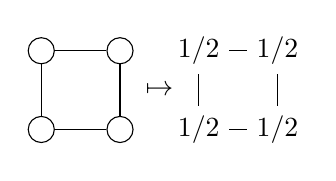
\begin{tikzpicture}[scale=0.5]
    \node[draw, circle] at(0,1)(s1){};
    \node[draw, circle] at(0,-1)(u1){};
    \node[draw, circle] at(2,1)(v1){};
    \node[draw, circle] at(2,-1)(t1){};
    \draw (s1) -- (u1) -- (t1) -- (v1) -- (s1);
    \node at(3,0){$\mapsto$};
    \node at(4,1)(s2){$1/2$};
    \node at(4,-1)(u2){$1/2$};
    \node at(6,1)(v2){$1/2$};
    \node at(6,-1)(t2){$1/2$};
    \draw (s2) -- (u2) -- (t2) -- (v2) -- (s2);
\end{tikzpicture}

\end{document}